%:
\documentclass[11pt, oneside]{article}   	% use "amsart" instead of "article" for AMSLaTeX format
\usepackage{geometry}                		% See geometry.pdf to learn the layout options. There are lots.
\geometry{letterpaper}                   		% ... or a4paper or a5paper or ... 
%\geometry{landscape}                		% Activate for rotated page geometry
%\usepackage[parfill]{parskip}    		% Activate to begin paragraphs with an empty line rather than an indent
\usepackage{graphicx}				% Use pdf, png, jpg, or eps§ with pdflatex; use eps in DVI mode
								% TeX will automatically convert eps --> pdf in pdflatex		
\usepackage{amssymb}
\usepackage{diagbox}
\usepackage{amsmath}
\usepackage{amsthm}
\usepackage{enumerate}
\usepackage{tikz}
\theoremstyle{definition}
\newtheorem*{defn}{Definition}
\newtheorem*{prop}{Proposition}
\newtheorem*{eg}{Example}
\newtheorem*{thm}{Theorem}
\newtheorem*{corol}{Corollary}
\newtheorem{ex}{Exercise}[section]
{\theoremstyle{plain}
\newtheorem*{rmk}{Remark}
\newtheorem*{rmks}{Remarks}
\newtheorem*{lt}{Last time}
}
\newtheorem*{lem}{Lemma}
\usepackage{color}
\newcommand{\pars}[1]{{\left ( {#1} \right )}}
\title{Machine Learning Beyond Function Approximation I: Nondeterministic PAC-learning}
\author{Xiyu Zhai, Alexander Rakhlin}
\date{}							% Activate to display a given date or no date

\begin{document}
\maketitle
\tableofcontents

\section{Introduction}

Recently deep learning has been a thing. But no theories. And deep learning is still no match for humans. What's missing?

Good applied theories should satisfy the following criterions,
\begin{itemize}
	\item simple. Convoluted descriptions lead to no clean theories;
	\item relevant. Machine learning theories are not studied for its own sake, so it's important to have relevance to
	\item insightful. Good theories can make predictions that could guide future experiments, instead of just explaining the known empirical success. A good set of assumptions should make it possible to draw insights and make predictions about future directions of experiments and engineering.
\end{itemize}

Theoretical Physics has been extremely successful in the light of these criterions, and we have yet to see the same level of success happening for theoretical machine learning. As Feifei Li commented, we are in a pre-Newton era of AI. If we compare physics with machine learning, machine learning is more difficult to establish elegant and effective theories due to
\begin{itemize}
	\item medium scaling. Scaling in machine learning is neither too big nor too small to allow simplification. Statistical Physics or astronomical Physics deals with a gigantic system with the number of particles being around the order of $10^{23}$ and things can be simplified with renormalization. Atomic Physics deals with a tiny system with only a few number of particles and things are simplified to be equations with several variables. Anything between is notoriously difficult in Physics. However, the scaling of deep learning is not as nice to simplify things to adapt either renormalization or precise analysis.
	\item incomplete information. Physics studies from a God's perspective, no loss of information when doing the calculation. However, machine learning deals with incomplete information on a daily basis. Informally, one can summarize using the following diagram, which shall reappear with more details,
	\begin{center}
		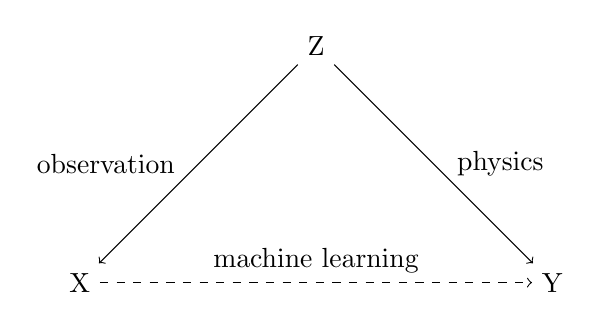
\begin{tikzpicture}
		  % Nodes
		  \node (Z) at (0,3) {Z};
		  \node (X) at (-3,0) {X};
		  \node (Y) at (3,0) {Y};

		  % Arrows
		  \draw[->] (Z) -- (X) node[midway, left=5pt] {observation}; % Solid arrow from Z to X
		  \draw[->] (Z) -- (Y) node[midway, right=5pt] {physics}; % Solid arrow from Z to Y
		  \draw[->, dashed] (X) -- (Y) node[midway, above] {machine learning}; % Dashed arrow from X to Y
		\end{tikzpicture}
	\end{center}

	The solid arrows are well-defined and easily represented by analytic functions, but the dashed arrow is often not well-defined and hard to be analytically represented as $Z \to X$ is not invertible. In computer vision, $Z$ is the complete physical world and $X$ is the projection of $Z$ to a certain camera and $Y$ is a certain well-defined quantity of the physical world. In natural language processing, $Z$ can be the meaning one wants to convey and $X$ is the actual word one speaks to convey the meaning and $Y$ is a certain aspect of the meaning $Z$.
\end{itemize}

\subsection{In this paper}
We extend the PAC-learning framework.

\subsection{Contributions}
hello

\subsection{Notations}

In machine learning, people tend to use $Y^X$ for the set of maps from $X$ to $Y$. Here we use $X \to Y$ instead for consistency. Our paper address problems lying the intersection of computer science, mathematics, and statistics. In computer science, the curry notion is $X\to Y$ and one use `:' for type annotation. In mathematics, one tends to write $f: X \to Y$. So it seems that $X\to Y$ would be a notation that comes close to all sides.

\section{Related Work}

Bayesian.

Compression. Ilya talks 

\section{Limitations of PAC-learning Framework}

In this section, we point out that the assumptions in the PAC-learning framework are too restrictive for many important applications. In fact, it might be too restrictive for most important applications.

\newcommand{\Input}{\mathcal{X}}
\newcommand{\Output}{\mathcal{Y}}
\newcommand{\InputDistribution}{\mathcal{P}}
\newcommand{\Expect}{\limits(\mathbb{E})}
\newcommand{\ExpectInput}[1]{\mathbb{E}_{#1 \sim \InputDistribution}}
\newcommand{\HypothesisClass}{\mathcal{H}}
\newcommand{\LearningAlgorithm}{\mathcal{A}}
\newcommand{\deformableTemplate}{\phi}
\newcommand{\DeformationSpace}{\Gamma}
\newcommand{\argmax}{\mathop{\operatorname{argmax}}}

Let $\Input$ be the input space, and $\Output$ be the output space, and we wish to learn a function $f_*$ from $\Input$ to $\Output$, called the ground truth. We are given $x_1, \dots, x_n$ sampled according to a distribution $\InputDistribution$, and also $y_1, \dots, y_n$ with $y_i=f_*(x_i)$, and we want to get a function $f$ such that

\[ \ExpectInput{x}l(f_*(x),f(x)) \]

is as small as possible.

Let $\HypothesisClass$ be a set of functions from $\Input$ to $\Output$, called the hypothesis class, we say that $\HypothesisClass$ is PAC-learnable if there exists an algorithm $\LearningAlgorithm$ that takes in a training set $S \in (\Input \times \Output)^n$ and returns $\LearningAlgorithm_S \in \HypothesisClass$ in polynomial time such that

\[ \ExpectInput{x}l(f_*(x), \LearningAlgorithm_S(x)) < \epsilon \]

Note that the hidden assumption is that functions in $\HypothesisClass$ can be computed in a ``straightforward'' manner. By ``straightforward'', we mean that the mathematical description gives directly a feasible way of computation, just like the description of neural networks gives directly a way to compute them in an acceptable amount of time, although it might not be optimal.

The problem with this setup is that it's too simplistic. In a sense, it is as naive as assuming all differential equations with analytic representation have analytic solutions.  Many important problems are naturally represented by a hypothesis class containing functions not straightforward to evaluate. Not taking these problems into consideration is somehow like not considering equations without an analytic solution, leading to the unavoidable large gaps between theories and practices.

Here are some examples that show that such problems do exist across different AI domains.

\paragraph{Example (Computer Vision, Image Recognition, Deformable Template Matching, Informal)} Image classification in computer vision is about using computers to tell the class of an image, i.e. $\Input$ being the space of images, and $\Output$ being a small set of categories. A reasonable simplification for many cases is that the process can be realized through deformable template matching. A deformable template is a map $\deformableTemplate$ from a deformation space $\DeformationSpace$ to the same image space $\Input$. Let $d_\Input$ be the natural metric on image space $\Input$, then we can construct a measure of the degree of an image fitting a template through

\[ s(\deformableTemplate, x) := \inf_{\gamma \in \DeformationSpace} d_\Input (x, \phi(\gamma)) \]

It's not as easy to compute as to define. $\DeformationSpace$ can be of very high dimensionality making it nearly impossible to evaluate $s(\deformableTemplate, x)$ faithfully.

Now suppose that we have a list of pairs of deformable template and category, say, $(\deformableTemplate_1, y_1), \dots, (\deformableTemplate_n, y_n)$, the ground truth can be given by

\[ f_*(x) = y_i \text{ where } i = \argmax_i s(\deformableTemplate_i, x) . \]

Evaluating $f_*$ is thus not straightforwardly easy.

For more concrete examples, we give a full mathematical characterization of the MNIST dataset in the appendix.

\paragraph{Example (Natural Language Processing, Word, Informal)}

% ... Continue with the rest of your document ...

\begin{defn}[]
	
\end{defn}

\section{Nondeterministic PAC-learning (NPAC-learning)}

The nondeterministic PAC-learning is trying to be an extension of PAC that deals with more cases, but not everything. We would like to point out there are more beyond the scope of this theory.

\newcommand{\Weight}{W}

\newcommand{\Configuration}{\Gamma}
\newcommand{\NondeterministicHypothesisClass}{\mathcal{H}(\Gamma,\mathcal{F})}
\newcommand{\StructureFunctionClass}{\mathcal{F}}

Let $\Configuration$ be a set called the configuration space, and $\StructureFunctionClass\subseteq(\Input\times \Output\times \Configuration \to \mathbb{R})$ be a set called the class of structure functions. We shall define the nondeterministic hypothesis class $\NondeterministicHypothesisClass$ as follows.

For each $f\in \StructureFunctionClass$ we define an energy function $e_f: \Input\times\Output\to \mathbb{R}$ as
\begin{equation}
	e_f(x,y):=\sup\limits_{\gamma\in \Configuration} f(x, y, \gamma),
\end{equation}
and we define a hypothesis function $h_f: \Input\to\Output$ as
\begin{equation}
	h_f(x)=\argmax\limits_{y\in \Output}e_f(x,y)
\end{equation}

For the above to be well-defined, one assumes that $\Output$ is finite and has a default ordering and $\argmax\limits_{y\in \Output}$ returns $y$ with the largest ordering if the global maxima are not unique.

Finally we define the nondeterministic hypothesis class as
\begin{equation}
	\NondeterministicHypothesisClass:=\{h_f:f\in \mathcal{F}\}
\end{equation}

\begin{rmk}
	We are still call it hypothesis class instead of concept class because there is no guarantee that the ground truth lies in this hypothesis class.
\end{rmk}

then

\begin{rmk}
	[Equivalence with Bayesian to the Limit] $h_w$ is equivalent to

	Let $\mu=\mu_\Input\times\mu_\Output\times \mu_\Configuration$ be a standard measure over $\Input\times\Output\times\Configuration$, let $P_\varepsilon$ be another distribution defined by
	$$p_\varepsilon(x,y,\gamma):=\frac{dP_\varepsilon}{d \mu}\Big|_{x,y,\gamma}=Ce^{f(x,y,\gamma;w)/ \varepsilon}$$

	where $C$ is a normalization constant.

	Given only $x\in\Input$, we have
	\begin{equation}
		p_\varepsilon(y|x)=\frac{
			\int_{\Configuration} p_\varepsilon(x,y,\gamma)d \mu_{\Configuration}(\gamma)
		}{
			\int_{\Output}\pars{\int_{\Configuration} p_\varepsilon(x,y,\gamma)d \mu_{\Configuration}(\gamma)} d \mu_{\Output}(y)
		}.
	\end{equation}

	As $\varepsilon \to 0$, and assuming that with $\epsilon$-margin, then

	\begin{equation}
		p_\epsilon(y|x) \to C 1_{y=h_w(x)}
	\end{equation}

	where $C$ might be as large as $\delta(0)$.
\end{rmk}

Consider the following diagram
\begin{center}
	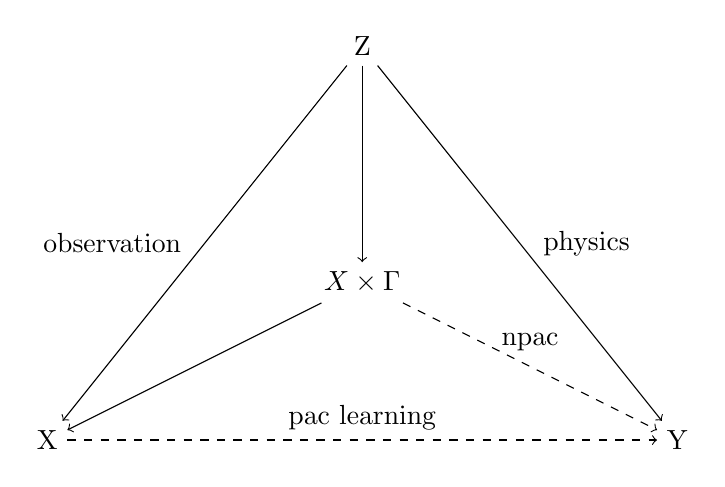
\begin{tikzpicture}
	  % Nodes
	  \node (Z) at (0,5) {Z};
	  \node (XGamma) at (0,2) {$X\times \Gamma$};
	  \node (X) at (-4,0) {X};
	  \node (Y) at (4,0) {Y};

	  % Arrows
	  \draw[->] (Z) -- (X) node[midway, left=5pt] {observation}; % Solid arrow from Z to X
	  \draw[->] (Z) -- (Y) node[midway, right=5pt] {physics}; % Solid arrow from Z to Y
	  \draw[->] (Z) -- (XGamma) node[midway, right=5pt]{}; % Solid arrow from Z to Y
	  \draw[->] (XGamma) -- (X) node[midway, right=5pt]{}; % Solid arrow from Z to Y
	  \draw[->, dashed] (XGamma) -- (Y) node[midway, above=2pt]{npac}; % Solid arrow from Z to Y
	  \draw[->, dashed] (X) -- (Y) node[midway, above] {pac learning}; % Dashed arrow from X to Y
	\end{tikzpicture}
\end{center}

The diagram suggests that it can be easier to construct a function from $X\times \Gamma$ to $Y$ then from $X$ to $Y$ because of additional information.

\section{Basic Function Properties}

\begin{prop}
	[Lipschitz] Suppose that $f$ is $L$-Lipschitz w.r.t $\Input$ then $e_w$ is $L$-Lipschitz w.r.t $\Input$.
\end{prop}

\begin{proof}
	Obvious by unravelling the definitions and note that $\sup$ keeps the Lipschitzness.
\end{proof}


% Content for this section ...

\section{Generalization Bound}

% Content for this section ...

\section{Select and Verify}

\subsection{Differentiable}

\subsection{Neural Network}

\section{Shape Theory}

% Content for this section ...

\appendix

\section{Description of Function Classes}

In machine learning theory, people just refer to function classes as mathematical sets, without further structures. For our purposes, this is not enough. So

\section{Mnist} 
Here we describe briefly a function in mathematical terms which we believe is the ground truth for the MNIST dataset. Details can be seen in appendix.

We take the convention that the fill of the digits is white and the background is black.

The image is represented by a $[0,1]$-valued $28\times 28$ matrix $I=(I_{ij})_{0\le i\le 27, 0\le j\le 27}$.

\begin{itemize}
	\item \textbf{digit one of the simplest kind}, which constitutes 95\% of all images of digit one.

A typical image looks like this:

[an image here]

Think about how it's drawn. The person when writing down a digit one like this has an ideal version in mind, a straight line that is almost vertical. So take $\Gamma_1$ to be the set of straight lines with slopes satisfying some easy constraint. Then we should define $\mathfrak{s}(x;\gamma)$ for $\gamma\in \Gamma_1$ such that
\begin{itemize}
	\item for "most" points over $\gamma$, it's surrounded by white pixels;
	\item for "most" non-white pixels, it's away from $\gamma$.
\end{itemize}

One choice could be
\begin{equation}
	\mathfrak{s}(x; \gamma)=a_1\int_{0}^1  \max_{(i,j)\in [27]\times[27]}1_{\|\gamma(t) - (i,j)\|_2 < \epsilon} I_{ij}dt
	-
	a_2\sum_{(i,j)\in [27]\times[27]} 1_{I_{ij}< 0.5}\text{dist}((i,j), \gamma)
\end{equation}

where $\epsilon$ is an appropriate small number and $a_1,a_2>0$ are appropriate coefficients.

In fact the function applies when $\gamma$ is any path, not necessarily a straight line. Formally it is defined over the path space (without basepoint) $\Gamma= M([0,1], [0,1]^2)$.

The dimensionality of the configuration space is 6, which can possibly be reduced to 5.

\item \textbf{digit seven of the simplest kind}.

A typical image looks like this:

[an image here]

Here we consider all continuous $\gamma:[0,2]\to [0,1]^2$ such that $\gamma|_{[0,1]}, \gamma|_{[1,2]}$ are straight line segments. Additionally, there should be some constraint on the positions of $\gamma(0), \gamma(1), \gamma(2)$ such that $\overline{\gamma(0)\gamma(1)}$ is very close to being horizontal, and $\overline{\gamma(1)\gamma(2)}$ should be roughly vertical downward.

The score function $\mathfrak{s}$ is the same.

The dimensionality of the configuration space is 6, which can actually be reduced to 5.

\item \textbf{digit zero}.

We consider smooth curves $\gamma:[0,L]\to [0,1]^2$ with arc length parametrization such that the mean curvature is always nonnegative, i.e.
\begin{equation}
	\|\gamma'(t)\|\equiv 1
\end{equation}
and
\begin{equation}
	\gamma''(t)\times \gamma'(t) \ge 0
\end{equation}

Additionally, we require that $\gamma(0)$ is very close to $\gamma(L)$.

We should also require that $\gamma$ is nondegenerate, which can be characterized by isoperimetric inequality.

All these $\gamma$ form $\Gamma_0$.

And we still use the same score funtion $\mathfrak{s}$.

\item \textbf{general case}. Fix a graph $G=(V,E)$. Give it a natural topological structure and identify each $e$ with $[0,1]$. For each $e\in E$, we give assign a $\sigma_e$ which is one of the following classes of curves:

\begin{itemize}
	\item nonconvex but not straight
	\item nonconcave but not straight
	\item straight.
\end{itemize}

We define the total space as
\begin{equation}
	\Omega_G = \left\{\gamma\in M(G, [0,1]^2): \forall e\in E, \gamma|_e\in \sigma_e\right\}.
\end{equation}

Then the configuration space $\Gamma_G$ is a subset of $\Omega_G$ such that it is given by a boolean function $s$ in the sense that
\begin{equation}
	1_{\Gamma_G}(\gamma)=s((\gamma(v))_{v\in V},((\gamma|_e'(0), \gamma|_e'(1), \text{dist}(\gamma|_e,\overline{\gamma|_e(0)\gamma|_e(1)})))_{e\in E})
\end{equation}
\end{itemize}


\end{document}